\documentclass[fleqn]{article}
\usepackage[spanish,es-noshorthands]{babel}
\usepackage[utf8]{inputenc} 
\usepackage[left=1cm, right=1cm, top=1.5cm, bottom=1.7cm]{geometry}
\usepackage{mathexam}
\usepackage{amsmath}
\usepackage{amsfonts}
\usepackage{amssymb}
\usepackage{multicol}
\usepackage{graphicx}

\ExamClass{
\includegraphics[height=16pt]{Images/logo-sed.png} Matemáticas $6^{\circ}$}
\ExamName{`Evaluación, Operaciones en $\mathbb{N}$'}
\ExamHead{
\includegraphics[height=16pt]{Images/logo-colegio.png} IEDAB}
\newcommand{\LineaNombre}{%
\par
\vspace{\baselineskip}
Nombre:\hrulefill \; Curso: \underline{603} \; Fecha: \underline{\hspace*{2.5cm}} \relax
\par}
\let\ds\displaystyle

\begin{document}
\ExamInstrBox{
Respuesta sin justificar mediante procedimiento no será tenida en cuenta en la calificación. Escriba sus respuestas en el espacio indicado. Tiene 45 minutos para contestar esta prueba.}
\LineaNombre
\begin{enumerate}
   \item Ordene los números usando $<$ o $>$ según el caso: 
      \begin{enumerate}
	 \item De menor a mayor los siguientes números: 6050, 6500, 6005, 6555, 40005\answer*[6pt]{Resp:}
	 \item De mayor a menor los siguientes números: 3040, 3400, 34000, 3004, 30400, 60404\answer*[6pt]{Resp:}
      \end{enumerate}
  \item En la finca de Jerónimo, hay tres corrales. En el primero hay 235 reses, en el segundo hay 37 reses y en el tercero 208 reses.¿Cuántas reses tiene Jerónimo en su finca?\noanswer
  \item Encuentre el valor de $x$ apropiado en cada caso para que sea verdadera la igualdad.
  \begin{enumerate}
  \begin{multicols}{2}
    \item $x+13=25$, \qquad  entonces $x=$\underline{\hspace*{24pt}}
  \item $12+x=27$, \qquad entonces $x=$\underline{\hspace*{24pt}}
  \item $9+x=9$, \qquad entonces $x=$\underline{\hspace*{24pt}}
  \item $(6+x)+15=30$, \qquad entonces $x=$\underline{\hspace*{24pt}}
  \end{multicols}
  \end{enumerate}
  \item Efectúe las siguientes operaciones
  \begin{enumerate}
  \begin{multicols}{2}
  \item $58-23=$
  \item $23-58=$
  \end{multicols}
    \item $5404-397=$\noanswer[.5in]
  \item $2306-1579=$\noanswer[.5in]
  \end{enumerate}
  \item En una escuela hay 23 alumnos en primer grado, 32 en segundo grado, 28 en tercero y 25 en cuarto grado. Si la escuela tiene un total de 132 alumnos y hay los 5 grados de básica primaria, ¿cuántos alumnos hay en quinto grado? \noanswer
          \newpage
  \item Efectúe las siguientes operaciones y compare sus resultados
  \begin{enumerate}
  \item $12\times (7+9)=$\noanswer[24pt]
  \item $(12 \times 7)+(12\times 9)=$ \noanswer[24pt]
  ¿Qué puede concluir?\noanswer[24pt]
  \end{enumerate}
   \item Busca el término desconocido e indica su nombre en las siguientes operaciones:
   \begin{enumerate}
   \item Adición,\quad $439+\underline{\hspace*{48pt}}=1206$ \qquad Nombre:\underline{\hspace*{96pt}} \noanswer[36pt]
   \item Sustracción, \quad $\underline{\hspace*{48pt}}-4208=523$\qquad Nombre:\underline{\hspace*{96pt}} \noanswer[36pt]
   \item Sustracción, \quad $908-\underline{\hspace*{48pt}}=569$ \qquad Nombre:\underline{\hspace*{96pt}} \noanswer[36pt]
   \item Multiplicación,\quad $432\times \underline{\hspace*{48pt}}=15552 $ \qquad Nombre:\underline{\hspace*{96pt}}\noanswer[36pt]
   \end{enumerate}
   \item Si Alberto vende camisas a \$18350 cada una, y el sábado vendió 12 camisas, cuánto dinero obtuvo de la venta de las 12 camisas?\noanswer
\begin{minipage}{.34\textwidth}
   \item \textit{Punto extra}: Complete el siguiente sudoku:
\end{minipage}
\begin{minipage}{.65\textwidth}
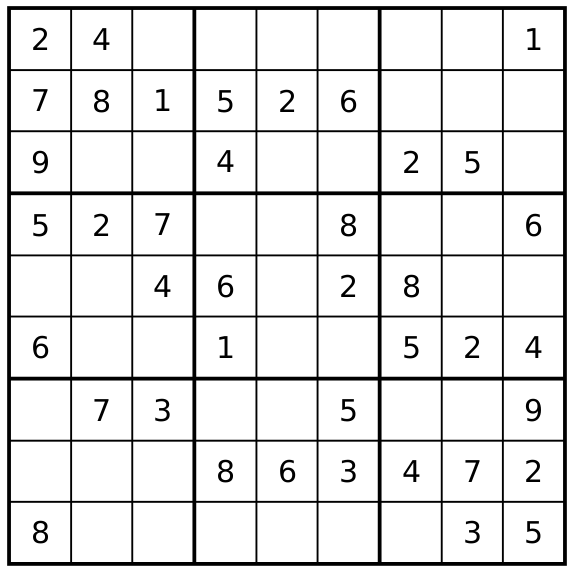
\includegraphics[scale=.25]{Images/sudoku02.png} 
\end{minipage}
\end{enumerate}
\end{document}
